\documentclass[../thesis.tex]{subfiles}

\begin{document}

\section{Methodology\label{sec:met}}
In this section, the details of an Eulerian--Lagrangian approach to perform the simulations is presented. Direct numerical simulations (DNS) of the background turbulent flow field has been employed together with a Lagrangian particle tracking (LPT) scheme to track the droplets. This  allows handling the flow--particle interaction, that is the particles (droplets) feel the flow via the viscous drag force. Moreover, the \emph{reverse} momentum coupling that represents particle--flow interaction is accounted for through an additional source term in the equations for the conservation of momentum in the flow field. Subsequently, the improved superposition method (ISM) that accounts for particle--particle aerodynamic interaction (AI) is discussed, followed by a technique to include the lubrication force in droplet AI. The combination of this analytical representation of droplet AI via the ISM and DNS of the flow, known as hybrid DNS (HDNS), is a widely established framework to simulate particle-laden turbulent flows. Later, the algorithm according to which the implementation works and the approach to include short-range lubrication effect in droplet AI is presented. Finally, the collision statistical indices that are employed to analyze the simulated droplet systems are defined.



\subsection{Background turbulent flow}
Following the previous studies \citep{TPARW13, APCRW14}, the turbulent flow is modeled using the Eulerian approach. The three-dimensional (3D) incompressible homogeneous isotropic turbulence is simulated in a cube of size $2\pi$ using a pseudo-spectral method. The fast Fourier Transform (FFT) applied to  the fluid velocity field implies periodicity at the domain boundaries in all three spatial directions. The Navier--Stokes (N--S) equations are discretized on a 3D uniform Cartesian mesh with $N$ equally spaced grid points. The governing equations are formulated in the rotational form
\begin{align}%%%%%%%%%%%%%%%%%%%%%%%%%%%%%%%%%%%%%
	\frac{\partial \boldsymbol{U}}{\partial t}&=\boldsymbol{U} \times  \boldsymbol{\omega} - \boldsymbol{\nabla}\left(\frac{P}{\rho}+\frac{\boldsymbol{U}^2}{2}\right)+\nu \boldsymbol{\nabla}^2\boldsymbol{U} + \boldsymbol{f}^{(b)} + \boldsymbol{f}^{(p)},\label{eq:1}\\
	\boldsymbol{\nabla \cdot U}&=0,\label{eq:2}
\end{align}%%%%%%%%%%%%%%%%%%%%%%%%%%%%%%%%%%%%%%%
where $\boldsymbol U(\boldsymbol x,t)$, $\boldsymbol \omega(\boldsymbol x,t)$, and $P(\boldsymbol x,t)$ are the velocity, vorticity, and pressure fields of the flow, respectively. The parameters $\rho$ and $\nu$ denote the density and kinematic viscosity of air, respectively. $\boldsymbol f^{(b)}(\boldsymbol x,t)$ is the body force acting on the fluid to maintain the turbulent flow. In the present study, we used a deterministic forcing scheme akin to that one developed by \citet{SMK94}. In this method, the energy of the first two shells, $0.5<|\boldsymbol{k}|<1.5$ and $1.5<|\boldsymbol{k}|<2.5$, is preset to be constant and consistent with the Kolmogorov energy spectrum, i.e.\ $|\boldsymbol{k}|^{-5/3}$. For a desired Reynolds number, these values cannot be set arbitrarily since for a statistically stationary turbulence, the average rate of energy input is equal to the average dissipation rate determined by the fluid viscosity. In the current simulations, the energy in these two shells is fixed to $E(1) = 0.55544$ and $E(2)=0.159843$, respectively. The added energy is distributed among 80 low-wavenumber modes specified by $|\boldsymbol{k}| <2.5$.

Moreover, the coupling term $\boldsymbol f^{(p)}(\boldsymbol x,t)$ represents the cumulative force per unit mass exerted by particles on the fluid and is defined as follows
\begin{equation}
\boldsymbol{f}^{(p)}\left(\boldsymbol{x},t\right)
=
-{M \over \rho}\sum\limits_{i=1}^{N_c} m_p^{(i)} \left({{\boldsymbol{U}^{(i)}-\boldsymbol{V}^{(i)}} \over \tau_p^{(i)}}+\boldsymbol{g} \right)\delta(\boldsymbol{x} - \boldsymbol{Y}^{(i)})
\label{eq:fpart}
\end{equation}
in which $m_p^{(i)}$, $\tau_{\text p}^{(i)}=2\rho_{\text p}(a^{(i)})^2/9\mu$, $\boldsymbol{Y}^{(i)}(t)$, and $\boldsymbol{V}^{(i)}(t)$ are the mass, Stokes inertial relaxation time, location, and velocity of particle $i$, respectively, where $i=1,\dots, N_{\text p}$. Additionally, the simplified notation $\boldsymbol{U}^{(i)}$ symbolizes the background flow velocity $\boldsymbol{U}(\boldsymbol{x},t)$ interpolated at the location of $i$-th particle: $\boldsymbol{Y}^{(i)}$. Also, $\boldsymbol{g}$ is the gravitational acceleration and $\delta$ is the Dirac delta function. In computation, function $\delta$ is mollified using one of the methods to projects \textcolor{red}{(project?)} momentum of droplets at their locations onto neighboring grid nodes \citep{GAR07}. The accuracy of different approaches for computing the mean interphase momentum transfer has also been discussed by \cite{RPW20}.
The parameter $M$ is a weighting factor defined as $M=N_r/N_c$  \citep{ELG94}, where $N_r$ and $N_c$ represent the number of real and computational particles (parcels), respectively. This factor enables, on the one hand, to reduce the computational cost of the simulations, especially at larger mass loadings, but on the other hand, it affects the accuracy of the model. Thus, in all simulations, if there were no computational constraints, we kept the value of $M=1$. In the case $M > 1$, each computational droplet represents $M$ real droplets. Such a treatment was proposed by \cite{ELG94} and it is known as super-droplet approach. Using this parameterization is unavoidable in simulations with small droplets at larger mass loadings on fine resolution meshes. 

In the two-way coupled systems, there is a net force on the fluid due to the particles. As a result, a mean flow must appear in the direction aligned with gravity. This effect violates the periodicity conditions on the boundaries of the domain and leads to instability in computations. To avoid the problem, the mean flow needs to be artificially attenuated in a way that guarantees the fidelity of the modeled processes. In the spectral space, the mean flow corresponds to the velocity mode at $|\boldsymbol{k}| = 0$. This Fourier mode was zeroed at each time step. Such a treatment is equivalent to applying a vertical counter pressure gradient. An alternative remedy to balance the mean air flow along the gravity direction is to add a force that corresponds to the weight of particles to the N--S equation. This method was employed both in point-particle approximation \citep{MON17} as well as particle-resolved simulations \citep{ZVLT21}.

It it important to note that two-way momentum coupling has not been considered ($\boldsymbol{f}^{(p)} = 0$) in the simulations of Subsections \ref{sec:lub} and \ref{sec:per} where the focus is on interacting droplets (disturbance velocity $\boldsymbol{u} \neq 0$) having lubrication effects. In the simulations, therefore, only diluted systems with low mass loadings of inertial droplets are modeled. Conversely, in the Subsection \ref{sec:2way}, where the effect of turbulence modulation by particles has been considered ($\boldsymbol{f}^{(p)} \neq 0$), the particles are not interacting with each other ($\boldsymbol{u} = 0$). In this way, each problem has been investigated separately in order to have a clear vision of the impact of each effect on the collision statistics of droplets using different assumptions for particle--particle and particle--flow interaction. 



\subsection{Lagrangian particle tracking}
Modeling of particle motion begins when the turbulent flow reaches a statistically stationary state. All particles are introduced into the domain at the same time instant. The initial locations are generated randomly enforcing uniform spatial distribution. Hereafter, the velocity and location of each particle are updated by integrating the equations of motion \citep{MR83} as follows
\begin{align}
\frac{\mathrm d \boldsymbol{V}^{(i)}}{\mathrm d \it t}&=-\frac{\boldsymbol{V}^{(i)}-\Big(\boldsymbol U^{(i)}+\boldsymbol{u}^{(i)}\Big)}{\tau_{\text p}^{(i)}}+\boldsymbol{g}\label{eq:3},\\
\frac{\mathrm d \boldsymbol{Y}^{(i)}}{\mathrm d \it t}&=\boldsymbol{V}^{(i)} \label{eq:4},
\end{align}
where $i=1,\dots, N_{\text p}$. Here, $\boldsymbol{u}^{(i)}$ is the disturbance velocity resulting from the presence of all particles, except particle $i$, sensed at the location of $i$-th particle. The velocity of particles in Equation~(\ref{eq:3}) is updated using the implicit fourth-order Adams--Moulton (AM3) scheme for $\boldsymbol{V}^{(i)}$ in conjunction with the explicit fourth-order Adams--Bashforth (AB4) for the composite flow field: $\boldsymbol{U}^{(i)}+\boldsymbol{u}^{(i)}$. Similarly, AM3 is used for integrating Equation~(\ref{eq:4}) to advance the location of particles in time. The multi-step schemes require keeping the record of velocities from previous time steps in memory arrays. The arrays are initialized with zeros. The initial condition for the velocity of each particle is the flow velocity at its location, to which its terminal velocity is added if the effect of gravity is considered. After each step of integration, periodicity is applied to the particles whose new locations fall outside the domain box; this simply means adding or subtracting the spectral length of the domain, $2\pi$, to or from their updated locations.

In our numerical model, two simplifying assumptions were made concerning rotation and deformation of droplets. The rotation of particles in turbulent flow can be considered from two different perspectives. First, as the motion of particles driven by randomly oriented vortical tubes relative to a fixed point of reference. We consider this type of motion in our model. Second, as the rotation enforced by torques generated by the turbulent flow or by interactions with other droplets in close proximity. Consequences of these effects can be safely neglected for cloud droplets due to the fact that the droplet radii are much smaller than the Kolmogorov length scale (by a factor of $\sim 50$) and their moments of inertia are relatively large (owing to the large particle-to-fluid density ratio). Thus, there is no efficient mechanism that forces the small droplets to rotate. 

The second simplifying assumption is that the droplets are treated as \emph{non-deformable} spherical bodies. For the considered ranges of Reynolds number and droplet sizes this approach accurately reflects the physics of the modeled processes and our simulation results do not lose their generality. A common measure used in the literature to quantify droplet deformation is the Weber number $(We)$. The number depends on the flow conditions and represents the relative importance of inertia and surface tension forces. For an isolated sphere the deformation is negligible if $We \ll 1$. In our simulations the maximal $We$ evaluated for 60~$\mu$m settling droplets (in absence of turbulence) is about 0.035. The presence of other particles has no significant effect here because their radial relative velocity is very low.



\subsection{Particle aerodynamic interactions}

Aerodynamic interaction (AI) among particles has been taken into account using the same formulation introduced by \cite{WAG05}. This approach has been later employed in combination with DNS of the background flow \citep{AGW07}, referred to as hybrid DNS (HDNS). In the this formulation, the disturbance velocity felt by $i$-th particle, $\boldsymbol{u}^{(i)}$, is computed by solving the linear system of equations
\begin{align}
\boldsymbol{u}_\text{HDNS}^{(i)}=
\underbrace{\sum_{j=1}^{N_{\text p}}}_{j\neq{i}}{\boldsymbol{u}_\text{St}}\Big(\boldsymbol{r}^{(ij)};a^{(j)},{\boldsymbol{V}^{(j)}}-\big({\boldsymbol{U}^{(j)}}+{\boldsymbol{u}_\text{HDNS}^{(j)}}\big)\Big),\quad
i=1,2,...,N_{\text p}.\label{eq:5}
\end{align}
Here ${\boldsymbol{u}_\text{St}}$ is the velocity disturbance induced by an arbitrary droplet $m_p^{(j)}$ at the location of droplet $i$. In the limit of low Reynolds number, ${\boldsymbol{u}_\text{St}}$ can be approximated by the analytical formula representing the solution of the Stokes equation for the perturbation flow induced by a single sphere of radius $a^{(j)}$ moving at ${\boldsymbol{v}}^{(j)}$
\begin{align}
\boldsymbol{u}_{\text{St}}\Big(\boldsymbol{r}^{(ij)};a^{(j)},{\boldsymbol{v}^{(j)}}\Big)&=\Bigg[\frac{3}{4}\frac{a^{(j)}}{{r}^{(ij)}}-\frac{3}{4}\bigg(\frac{a^{(j)}}{{r}^{(ij)}}\bigg)^{3}\Bigg]\frac{\boldsymbol{r}^{(ij)}}{({r}^{(ij)})^2}(\boldsymbol{r}^{(ij)}\boldsymbol{\cdot}\boldsymbol{v}^{(j)}) \nonumber\\
&+ \Bigg[\frac{3}{4}\frac{a^{(j)}}{{r}^{(ij)}}+\frac{1}{4}\bigg(\frac{a^{(j)}}{{r}^{(ij)}}\bigg)^{3}\Bigg]\boldsymbol{v}^{(j)},\quad
i=1,2,...,N_{\text p},\label{eq:6}
\end{align}
where $\boldsymbol{r}^{(ij)} \equiv \boldsymbol{Y}^{(i)}-\boldsymbol{Y}^{(j)}$ is the vector connecting centers of particles $j$ to $i$, and its magnitude is $\mathit{r}^{(ij)}=\|\boldsymbol{r}^{(ij)}\|$. As it transpires from Equations~(\ref{eq:5}) and (\ref{eq:6}), the flow disturbance acting on each particle is a linear function of the composite velocity field, ${\boldsymbol{U}^{(j)}}+{\boldsymbol{u}^{(j)}}$, which implicitly depends on the disturbance velocities of all other particles. Consequently, by moving all unknown disturbance velocities, $\boldsymbol{u}^{(j)}$, to the left-hand side of Equation~(\ref{eq:5}), the resulting system of equations in block matrix notation is
\begin{equation}
\underbrace{
{\begin{bmatrix}
{\boldsymbol I_3} & \cdots & {\boldsymbol \alpha^{(1,j)}} & \cdots &{\boldsymbol \alpha^{(1,N_{\text p})}} \\
\vdots &\ddots &\vdots &\ddots &\vdots \\
{\boldsymbol \alpha^{(i,1)}} & \cdots & {\boldsymbol \alpha^{(i,j)}} & \cdots &{\boldsymbol \alpha^{(i,N_{\text p})}}\\\vdots &\ddots &\vdots &\ddots &\vdots \\
{\boldsymbol \alpha^{(N_{\text p},1)}} & \cdots & {\boldsymbol \alpha^{(N_{\text p},j)}} & \cdots &{\boldsymbol I_3}
\end{bmatrix}}}_{\boldsymbol A}
{\begin{pmatrix}
\boldsymbol{u}_\text{HDNS}^{(1)}\\\vdots\\\boldsymbol{u}_\text{HDNS}^{(j)}\\\vdots\\\boldsymbol{u}_\text{HDNS}^{(N_{\text p})}\end{pmatrix}}
= (\boldsymbol A - \boldsymbol I_{N_{\text p}})
{\begin{pmatrix}\boldsymbol{V}^{(1)}-\boldsymbol{U}^{(1)}\\\vdots\\\boldsymbol{V}^{(j)}-\boldsymbol{U}^{(j)}\\\vdots\\\boldsymbol{V}^{(N_{\text p})}-\boldsymbol{U}^{(N_{\text p})}
\end{pmatrix}}
\label{eq:7},
\end{equation}
in which ${\boldsymbol \alpha^{(i,j)}}$ are $3\times3$ symmetric matrices, and $\boldsymbol I_3$ is the identity matrix while $\boldsymbol I_{N_{\text p}}$ is a diagonal matrix with $\boldsymbol I_3$'s on the main diagonal (see \citet{TPARW13} for details). Accordingly, this system has $3N_{\text p}$ inseparable equations in scalar form. At each time step it is solved iteratively by means of a parallel solver developed based on the generalized minimal residual method, GMRES \citep{TPARW13}. In practice, the matrix of coefficients is sparse since it is not necessary to consider interactions among all particles in the computational domain. This assumption is justified because the disturbance velocity induced by the particle decays as $1/r$ when $r\to\infty$, thus the effect of far-field aerodynamic interactions on the local interaction of two nearby particles can be safely neglected. Therefore, only perturbations due to droplets inside a spherical vicinity of each droplet are considered. The radius of this sphere is $H_{\text{tr}}\times a^{(j)}$, where $H_{\text{tr}}$ is a dimensionless truncation factor; hence, the larger the particle, the larger the neighborhood scanned for perturbing droplets. Conducting a sensitivity analysis on the influence of truncation radius, \citet{AGW07} demonstrated that considering perturbations of particles outside a truncation sphere with $H_{\text{tr}}=30$ does not make significant changes in collision statistics. Still, to more inclusively consider the neighborhood around each droplet, $H_{\text{tr}}=50$ is used in this study.

Among many numerical methods, HDNS is the one that allows us to quite accurately represent the many-body interactions among widely separated particles. This desirable feature is important, especially for modeling systems with a large number of droplets. It is worth recalling that HDNS was used in several previous studies for modeling systems that are relevant to typical atmospheric clouds \citep{WAKG05,AGW07,WAG07,WARG08,WRGHJ09}. Nevertheless, it should be pointed out that HDNS does not accurately represent the short-range lubrication forces. The method fails when the gap between particles is significantly smaller than the particles radii. This shortcoming is an indirect effect of using the ISM \citep{WAG05} to construct the numerical algorithm for computing particle drag.

\begin{figure}%----------- F I G U R E ----------
\center
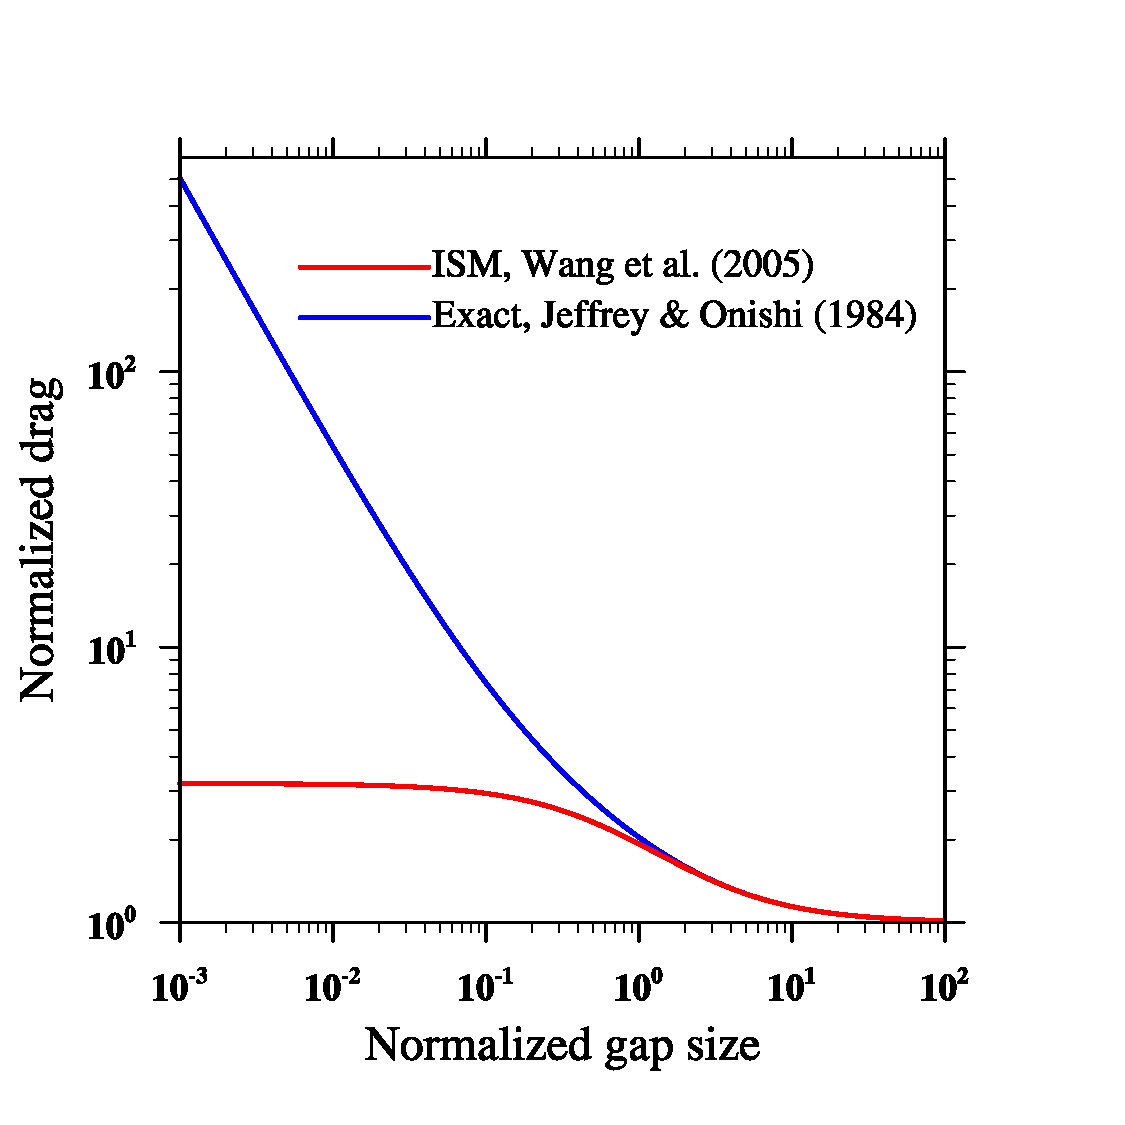
\includegraphics[width=0.6\textwidth]{../figs/JFM/fig1.pdf}
\caption{Normalized drag force (resistance) acting on two same-size spherical particles, whether approaching or receding, along their line of centers as a function of nondimensional gap between their surfaces.}
\label{Fig1}
\end{figure}%------------------------------------

The discrepancy can be quantitatively evaluated in a simplified case of two spheres in translational motion. In Figure~\ref{Fig1}, the normalized drag force, $F/-6\pi\mu a V$, acting on two droplets approaching to or receding from each other in a fluid of the dynamic viscosity $\mu$ at the velocity $V$ along their center-line are shown at various dimensionless gap distances: $\xi \equiv h/a$, where $h$ is the size of the gap between the surfaces of two particles.  In the figure, the exact analytical prediction of drag force \citep{JO84} indicates that the resistance asymptotically grows as the gap distance decreases. This, however, is valid only until the separation distance between the droplets would be of the order of the mean free path of air molecules beyond which the molecular nature of the fluid becomes important \citep{SK96}. Comparison of these analytically predicted forces with those obtained from the improved superposition method \citep{WAG05} shows that ISM does not yield an accurate representation of lubrication forces between two droplets when their gap distance is comparable to their average radii, i.e. $\xi < 1$. To overcome this problem, a new numerical approach is proposed here in which the standard HDNS is only used to represent the interactions between widely separated droplets while the drag of nearly touching droplets is computed using the exact analytical solution derived by \citet{JO84}. This strategy is somewhat similar to the one proposed by \citet[Equation 2.18 therein]{DBB87}.


\begin{figure}%----------- F I G U R E ----------
\centering
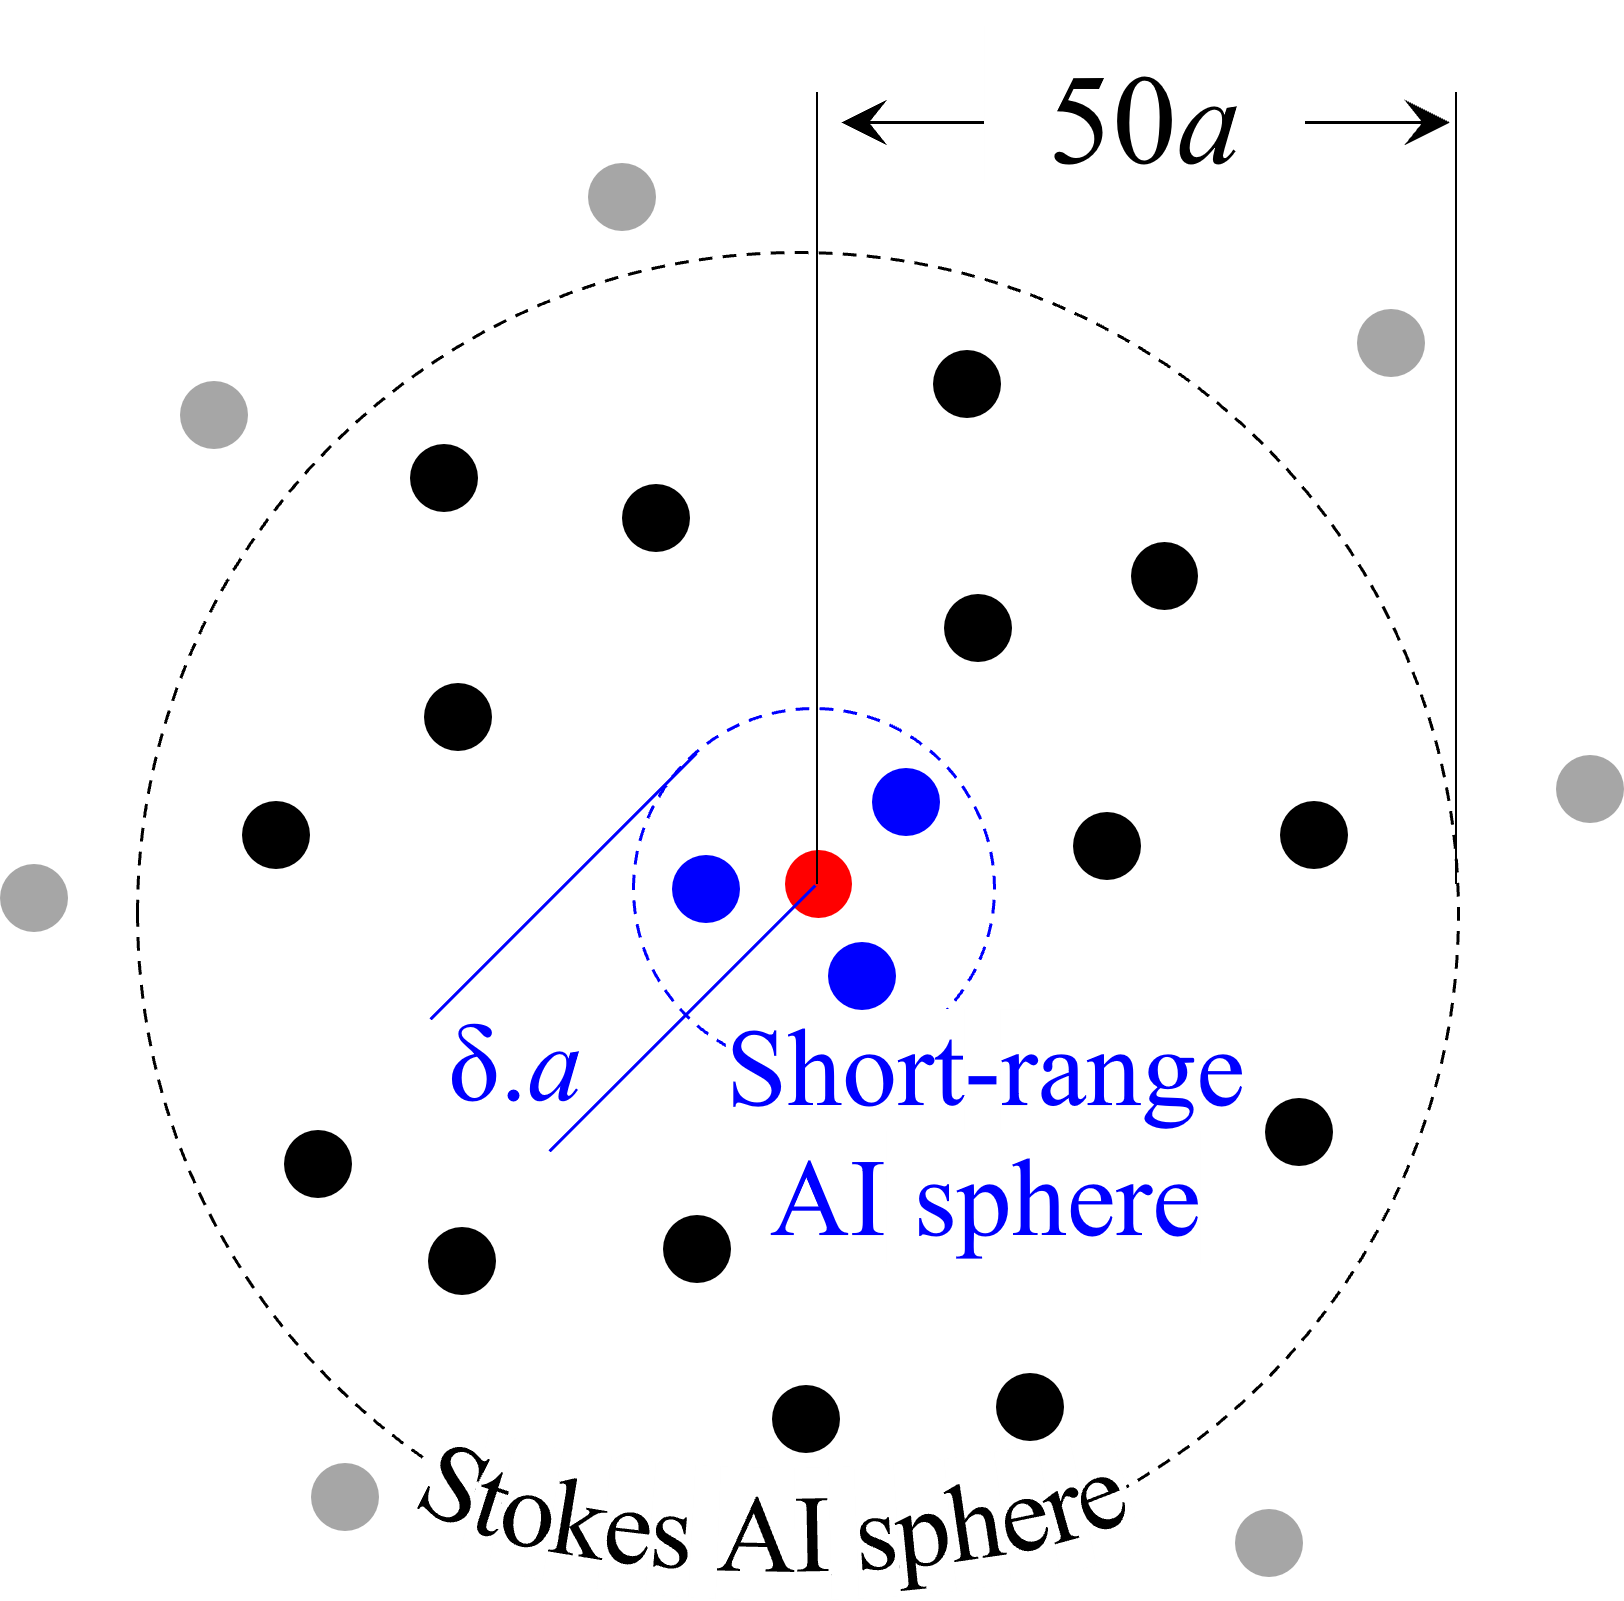
\includegraphics[width=0.5\textwidth]{./figs/PPAM/2/CP022_fig2.png}
\caption{The two spherical regions scanned around every particle (red) for neighboring particles interacting from short (blue) and long (black) distances}
\label{method}
\end{figure}%------------------------------------

To include lubrication effects, a border between the short- and long-range interaction need to be specified. Figure~\ref{method} shows a group of interacting particles. There are two spherical regions that define different approaches to represent aerodynamic interactions. (i) For particles closer than $\delta a$, exact analytical solutions \cite{JO84} are employed to accurately represent the lubrication forces. These solutions are in forms of infinite series and hence it is extremely time-consuming to calculate forces for every interacting pair at every time step. Instead, in the current implementation the forces are tabulated as functions of separation distance at the beginning of the simulation and for every instance the forces are interpolated from the tables. (ii) For particles interacting from a larger distance, $\delta a < r \leq 50a$, the superposition (HDNS) approach is used \citep{WAG05,AGW07}. For most of the cases analyzed here, short-range interactions \citep{JO84} are considered when the minimum distance between the surfaces is less than or equal to their mean radius, i.e.~$\delta=3$. This is the characteristic distance below which the superposition method loses its accuracy (see Figure~\ref{Fig1}). For particles that are considerably distant, $r>50a$, aerodynamic interaction is negligible (see Section 4.2 in \cite{AGW07}). (a lot of repetition)

In the new approach the disturbance velocity acting on $i$-th droplet is a superposition of two components
\begin{equation}
\boldsymbol{u}^{(i)}
=
\boldsymbol{u}^{(i)}_{\text{HDNS}} + \boldsymbol{u}^{(i)}_{\text{LUB}}.
\end{equation}
The first (long-range) component is evaluated using the HDNS algorithm with a modification that excludes the pairs separated at distances shorter than some preset normalized separation distance $s = \delta$, where $s \equiv r/a = \xi + 2$. According to this, $\delta$ marks the matching point where we switch between the short- and long-range interaction (see Figure \ref{method}). The second (short-range) component is only computed for all nearby pairs whose separation is $s\le\delta$ using the exact analytical formula derived by \citet{JO84}. 


In most of simulations $\delta=3$ was used. This means that the numerical method switches from HDNS to the exact solution when the gap size between droplet surfaces is smaller than the average size of the droplets radii. Sensitivity study of the modeled collisional statistics for different $\delta$ was also carried out and the results are presented and discussed. Contrary to other numerical models, the new approach allows to simultaneously include two effects, namely many-body interaction and lubrication forces. The only assumption made is that the binary interactions between nearby particles are not affected by the presence of other particles. This simplification has a rather negligible impact on the modeled systems, since the magnitude of short-range lubrication forces significantly exceeds the magnitude of interaction forces between particles separated by more than $s = 3$. While the lubrication forces can be influenced by many-body interactions, such a scenario is unlikely in dilute systems such as those considered in this study.

The forces acting on two nearby particles in the Stokes approximation are expressed in terms of the resistance matrix \citep{JO84}
\begin{equation}
\frac{1}{3\pi \mu(a_\alpha+a_\beta)}
{\begin{pmatrix}
{\boldsymbol{F}^{(1)}_{\text{LUB}}} \\
{\boldsymbol{F}^{(2)}_{\text{LUB}}}
\end{pmatrix}}
=
\begin{pmatrix}
{\boldsymbol{u}^{(1)}_{\text{LUB}}} \\
{\boldsymbol{u}^{(2)}_{\text{LUB}}}
\end{pmatrix}
=
\begin{bmatrix}
\boldsymbol{A}_{11} & \boldsymbol{A}_{12} \\
\boldsymbol{A}_{21} & \boldsymbol{A}_{22}
\end{bmatrix}
\begin{pmatrix}
\boldsymbol{V}^{(1)} - \boldsymbol{U}^{(1)} \\
\boldsymbol{V}^{(2)} - \boldsymbol{U}^{(2)}
\end{pmatrix},
\label{eq:8}
\end{equation}
where each component of the resistance matrix, $\boldsymbol{A}_{\alpha\beta}$, is a nondimensional second-rank tensor consisting of resistance functions $X^{\boldsymbol{A}}_{\alpha\beta}(s,\lambda)$ and $Y^{\boldsymbol{A}}_{\alpha\beta}(s,\lambda)$ that depend on the dimensionless separation distance and particles radius ratio $\lambda={a_2}/{a_1}$. In this thesis, only monodisperse systems are modeled, hence $s=r/a$ and $\lambda=1$. Moreover, the effect of particle rotation is not considered, therefore, torques and other rotational terms are already excluded from the resistance matrix in Equation~(\ref{eq:8}). Defining particle velocity relative to the background flow $\boldsymbol{v}^{(\beta)}\equiv\boldsymbol{V}^{(\beta)}-\boldsymbol{U}^{(\beta)}$, each tensor multiplication in Equation~(\ref{eq:8}) takes the following form
\begin{equation}
\boldsymbol{A}_{\alpha\beta}\:\boldsymbol{v}^{(\beta)}
=
X^{\boldsymbol{A}}_{\alpha\beta}\frac{\boldsymbol{r}}{r^2}\Big(\boldsymbol{r \cdot v}^{(\beta)}\Big)
+
Y^{\boldsymbol{A}}_{\alpha\beta}\bigg(\boldsymbol{v}^{(\beta)}-\frac{\boldsymbol{r}}{r^2}\Big(\boldsymbol{r \cdot v}^{(\beta)}\Big)\bigg),
\label{eq:9}
\end{equation}
where $\boldsymbol{r}\equiv\boldsymbol{Y}^{(2)}-\boldsymbol{Y}^{(1)}$. 
The first term is related to the drag force due to the squeezing motion of spheres along the line connecting their centers. The drag enforced by the shearing motion of spheres perpendicular to the line connecting their centers is handled by the second term. The resistance coefficients $X^{\boldsymbol{A}}_{\alpha\beta}(s,1)$ and $Y^{\boldsymbol{A}}_{\alpha\beta}(s,1)$ can be computed analytically using the procedure of twin multipole expansion developed by \cite{JO84}. The method is rather complex because the coefficients are given in terms of infinite series summations. Moreover, each term of the series can be determined only by solving complex recurrence relations. Further, the convergence rate of the series varies and depends on the specific configuration of the system such as the relative locations of the spheres. To obtain a satisfactory precision, more terms are needed when the particles are in proximity. Due to high complexity, the method cannot be used efficiently for modeling systems with many pairs of particles. Therefore, in our simulations the coefficients were pre-tabulated and then interpolated on the fly using the Bulirsch--Stoer rational interpolation algorithm: \texttt{ratint.f77} \citep{PTFV92}. This interpolation scheme has been adopted for a specific range of separation distances ``$s$'' since, as it is shown in Figure~\ref{Fig1}, the drag resistance resulting from the Stokes solution tends to infinity when $\xi \to 0$. In real applications this resistance coefficient is lower since the continuum assumption of the fluid breaks down when the gap is of the order of mean free path of air molecules \citep{SK96}. Besides, there would be potential numerical instabilities as a result of extremely large drag forces if the gap between droplets were extremely small. To address these problems, we made use of the ``collision gap model'' proposed by \citet{HJ70}. Namely, the algorithm for collision detection has been modified in a way that collision between two particles is assumed even if the minimum gap between their surfaces is greater than zero but smaller than $\epsilon_R$. In other words, the collision radius is slightly enlarged to $R=(2+\epsilon_R)a$, where $\epsilon_R=10^{-3}$. To assess sensitivity of our approach, we performed a set of test simulations with droplets of radii 40~$\mu$m using different values of $\epsilon_R$ in the range $(0.25-2.5)\times10^{-3}$. Based on the obtained results, not presented here, we conclude that this approach guarantees the numerical stability of the code while the differences in collision statistics are within statistical uncertainty. It should be added that after collisions, one of the particles is relocated and the problem with the large drag force acting on the particles is eliminated.



\subsection{Simulation algorithm}

\begin{figure}%----------- F I G U R E ----------
\centering
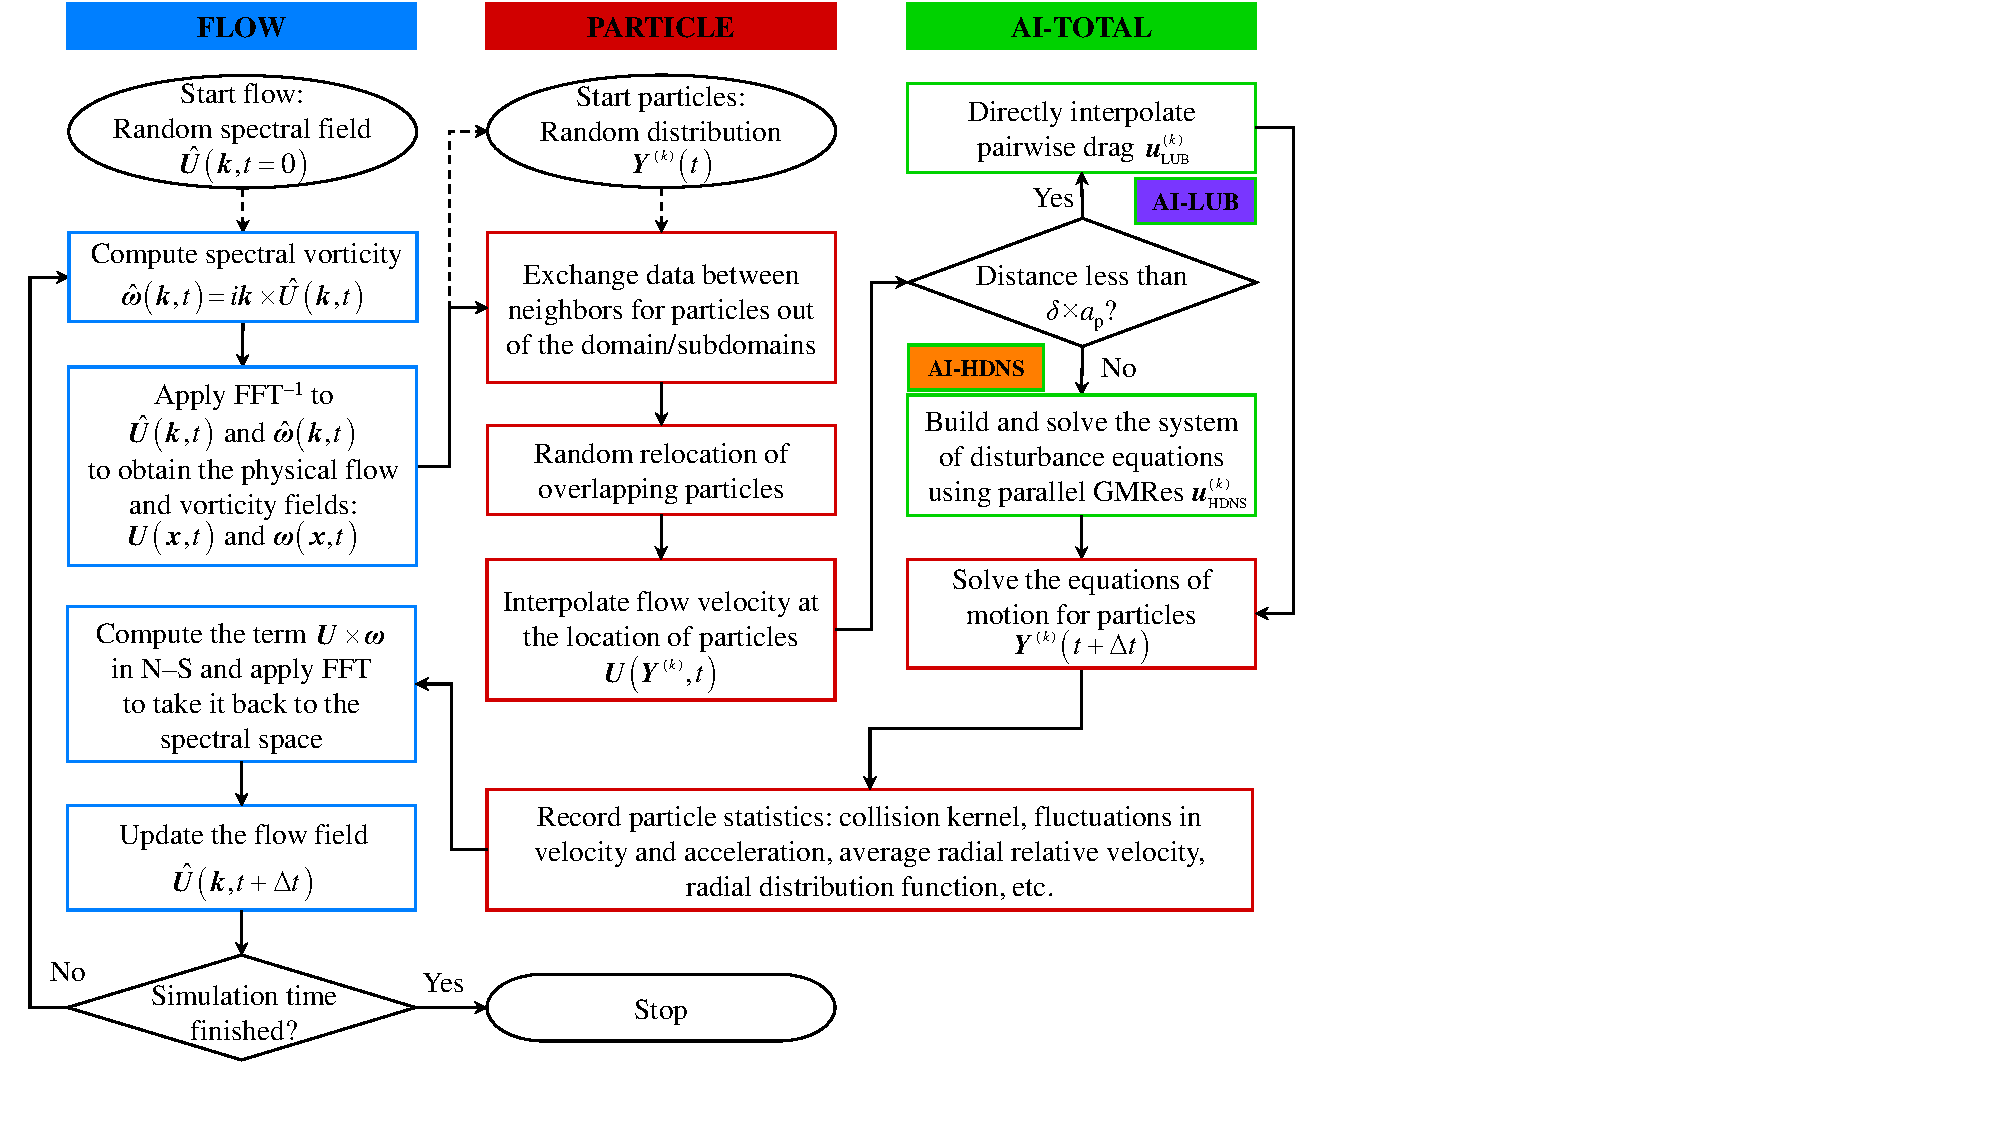
\includegraphics[trim=5mm 10mm 115mm 0mm, clip, width=\textwidth]{./figs/PPAM/1/CP022_fig1.pdf}
\caption{Schematic diagram of the simulation algorithm. The colors mark time measurements related to the flow, particles, and AI forces.}
\label{alg}
\end{figure}%------------------------------------
Figure~\ref{alg} presents the order in which the algorithm performs computations. Three major parts of simulation methodology, being related to the evolution of the flow, tracking the particles, and computing AI forces, are marked using different colors. The particle tasks are carried out locally within each subdomain and data exchange is conducted between neighboring subdomains. The main particle tasks unrelated to handling AI include solving the equations of motion (Equations~\ref{eq:3} and \ref{eq:4}), interpolation of the turbulent flow at droplet locations, transferring particle data to a neighboring subdomain when they cross subdomain or domain boundaries (i.e.~imposing periodicities), and collecting particle statistics such as collision kinematics (average relative velocity and distribution) as well as dynamics (collision rate), root mean square in velocity fluctuations,~etc. Also, two major operations are needed to compute particle aerodynamic interaction, including generation and solving the system of equations that yields AI among the particles (Equation~\ref{eq:7}) and the calculation of lubrication forces from analytical solutions (Equation~\ref{eq:8}).



\subsection{Collision statistical indices}
The new implementation will be used to compute collision statistics of monodisperse particle systems relevant to atmospheric clouds. The main focus is on two-point particle statistics such as the radial distribution function (RDF) and the radial relative velocity (RRV). These quantities were computed ``on the fly'' during simulations and then averaged over time at a postprocessing stage. The radial relative velocity between two particles is defined as $w_\text{r}=\boldsymbol{w\cdot r}/r$, where $\boldsymbol{w}=\boldsymbol{V}^{(2)}-\boldsymbol{V}^{(1)}$ is their relative velocity vector. This quantity is a function of separation distance $r$ and can be computed for every pair of droplets in the computational domain. In further analysis, we only consider the absolute value of the average RRV, i.e. $\langle|w_\text{r} (r/R)|\rangle$ for all particle pairs computed for a sufficiently long simulation time: in most cases 100$T_e$. The spherical neighborhood that is scanned around each droplet is limited to $1\leq r/R\leq10$. This range is divided into 180 spherical shells of thickness $\delta_\text{sh}=0.05R=0.1a$.

A similar method was used to compute the radial distribution function. The RDF characterizes preferential concentration, or clustering \citep{BIC15}, of the particles at different length scales. For a system with a monodisperse set of droplets, RDF is defined as
\begin{equation}
g_\text{r} (r/R; t)=\frac{n_\text{pair}/V_\text{sh}}{\frac{1}{2}N_{\text p}(N_{\text p}-1)/V_\text{box}},
\end{equation}
where $V_\text{box}$ is the volume of the computational domain and $V_\text{sh}(r/R)$ is the volume of each spherical shell within which fall $n_\text{pair}(r/R; t)$ pairs of droplets.

The product of the RRV and RDF of aerodynamically non-interacting particles at contact, i.e. $r=R$, is proportional to the kinematic collision kernel, $\Gamma^\text{K}$, namely
\begin{equation}
\Gamma^\text{K}=2\pi R^2 \; \langle|w_\text{r} (r=R)|\rangle \; g_\text{r} (r=R).
\label{eq:32}
\end{equation}
In NWP, the collision kernel is central for mathematical models that represent grid scale cloud processes and precipitation formation. An alternative formulation for $\Gamma$, the so-called dynamic collision kernel, can be evaluated by counting collisions of droplets, $N_c(t)$, in the entire computational box for a given time period. Having the volumetric rate of collisions, $\dot{N}_c$, the dynamic collision kernel, $\Gamma^\text{D}$, can be evaluated using the formula \citep{ARWG08}:
\begin{equation}
\dot{N}_c=\Gamma^\text{D} \frac{1}{2}N_{\text p}(N_{\text p}-1)/V_\text{box}.
\label{eq:33}
\end{equation}
The assessment of uncertainty in the dynamic collision kernel is explained in \citep{RPAGW13}. The dynamic formulation of the collision kernel is based on the actual collision events and therefore is more accurate. Besides, the effect of aerodynamic interactions is inherently accounted for, while the standard definition of kinematic collision kernel, Equation~(\ref{eq:32}), needs to be revised for that purpose. This is largely due to the \textit{non-overlapping droplets} condition applied to the pairs that collide. After each collision one of the droplets must be relocated, resulting in a particle-free zone behind the collision sphere of the collided pair. To address this issue, \citet{WAKG05} proposed a correction based on subtracting the influx through the surface area of each shell that is in shadow of the collision sphere from the total influx. Such a treatment is justified since no particles can be found behind the collision sphere due to the imposed relocation condition. Consequently, the resulting correction factors for $g_\text{r} (r/R)$ and $\langle|w_\text{r} (r/R)|\rangle$ in each spherical shell, with inner and outer radii of $r_1/R$ and $r_2/R$, are
\begin{equation}
C_g\left(\frac{r_1}{R},\frac{r_2}{R}\right)=\frac{1}{2}+\frac{1}{2}\frac{\left(\left(r_2/R\right)^2-1 \right)^{3/2}-\left(\left(r_1/R\right)^2-1 \right)^{3/2}}{\left(r_2/R\right)^3-\left(r_1/R\right)^3}, \label{eq:34}
\end{equation}
\begin{equation}
C_w\left(\frac{r_1}{R},\frac{r_2}{R}\right)=\left(
1-\frac{3}{2}\frac{r_2/R-r_1/R}{\left(r_2/R\right)^3-\left(r_1/R\right)^3} \middle)\right/ C_g\left(\frac{r_1}{R},\frac{r_2}{R}\right),\label{eq:35}
\end{equation}
respectively, such that the corrected RDF and RRV will be obtained by
\begin{align}
g_\text{r}^\text{c} (r/R)&=g_\text{r}/C_g,\label{eq:36} \\
\langle|w_\text{r}^\text{c} (r/R)|\rangle&=\langle|w_\text{r}|\rangle/C_w,\label{eq:37}
\end{align}
and the kinematic collision kernel
\begin{equation}
\Gamma^\text{K}=2\pi R^2 \; \langle|w_\text{r}^\text{c} (r=R)|\rangle \; g_\text{r}^\text{c} (r=R).\label{eq:38}
\end{equation}
From now on, the superscript ``c'' for corrected RRV and RDF will be dropped.



%\bibliographystyle{bibstyle}
%\bibliography{references}
\newpage
\end{document}
